\chapter{Neural Networks Compression}
-Model compression encompasses a family of techniques aimed at reducing the computational and memory demands of neural networks while preserving, as much as possible, their predictive performance. These methods are typically applied at the level of layers, submodules, or parameter groups and introduce explicit trade-offs between efficiency metrics and model accuracy. Key objectives include reducing model size, lowering inference latency, decreasing memory bandwidth usage, and accelerating both training and deployment, particularly in resource-constrained environments.

A notable characteristic of modern deep learning models is their heavy overparameterization. In such regimes, compression does not merely remove redundancy but can also act as an implicit form of regularization, mitigating overfitting and occasionally improving generalization performance. This phenomenon has been observed across a variety of architectures, especially in large-scale transformer-based models.

Among the most widely adopted compression strategies are \emph{knowledge distillation}, \emph{quantization},\emph{pruning} and \emph{low-rank factorization}. Pruning methods remove parameters, neurons, attention heads, or entire structural components deemed redundant or unimportant according to some saliency criterion, thereby inducing sparsity in the network. Quantization reduces numerical precision by representing weights, activations, or gradients with fewer bits, leading to significant gains in memory efficiency and hardware throughput. Knowledge distillation transfers information from a high-capacity teacher model to a smaller student model by matching output distributions or intermediate representations, enabling compact models to retain much of the teacher’s behavior. Low-rank factorization exploits linear dependencies in weight matrices by decomposing them into products of smaller matrices, effectively reducing parameter count and computational complexity without altering the overall network topology.

These techniques are not mutually exclusive and are frequently combined in practice. Hybrid compression pipelines leverage their complementary strengths to achieve higher compression ratios and better efficiency–accuracy trade-offs than any single method alone.

\section{Knowledge Distillation}
\label{sec:kd_introduction}

The rapid advancement of Deep Neural Networks (DNNs) has revolutionized fields like Computer Vision (CV) and Natural Language Processing (NLP). Models such as Transformers, and more recently, Large Language Models (LLMs) and Vision Foundation Models, have achieved state-of-the-art performance on a vast array of tasks. However, this success comes at a significant cost: these models are often massive, containing billions or even trillions of parameters \cite{Kaplan2020}. This over-parameterization, while beneficial for performance, creates substantial challenges for practical deployment, especially in resource-constrained environments like mobile devices or edge computing hardware. The high computational and memory requirements lead to prohibitive inference latency and energy consumption, motivating the critical need for \textbf{model compression}.

Several techniques have been developed to address this challenge, including pruning, quantization, low-rank factorization, and the design of efficient network architectures. Knowledge Distillation (KD) stands out as a powerful and distinct paradigm within this landscape.

\subsection{The Core Concept: The Teacher-Student Framework}

Knowledge Distillation, a concept popularized by Hinton et al. \cite{Hinton2015}, is a compression technique that trains a smaller, more efficient "student" network to mimic the behavior of a larger, pre-trained, and more powerful "teacher" network. Unlike methods like pruning or quantization that modify the architecture or parameters of an existing model, KD transfers the "knowledge" from one model to another.

The fundamental workflow, illustrated in Figure \ref{fig:teacher_student_framework}, follows a simple principle:
\begin{enumerate}
    \item \textbf{The Teacher Model}: A large, cumbersome model that has already been trained on a massive dataset and has achieved high performance. Its primary role is to act as a source of rich, generalized knowledge.
    \item \textbf{The Student Model}: A smaller, lightweight model with a more efficient architecture (e.g., fewer layers or channels). This is the model intended for final deployment.
    \item \textbf{Knowledge Transfer}: The student model is trained not only on the ground-truth labels of the dataset but also to replicate the outputs of the teacher model. This process distills the teacher's nuanced understanding into the more compact student architecture.
\end{enumerate}

\begin{figure}[htbp]
    \centering
    % Placeholder for the diagram. You can recreate or use the one from the survey.
    % In the survey, this corresponds to Figure 1.
    
\includegraphics[width=0.8\textwidth]{Figures/figure1_teacher_student.pdf}
    \caption{The general Teacher-Student framework for Knowledge Distillation. The student learns to mimic the knowledge extracted from the pre-trained teacher, in addition to learning from the input data. (Diagram inspired by Mansourian et al., 2025).}
    \label{fig:teacher_student_framework}
\end{figure}

\subsection{The Motivation: Beyond Hard Labels}

A key insight behind Knowledge Distillation is the concept of **"dark knowledge."** When a model is trained conventionally, it learns to predict "hard labels" (e.g., a one-hot vector like `[0, 0, 1, 0]`). This approach discards a significant amount of information that the model has learned.

For instance, a well-trained image classifier, when shown a picture of a cat, might not just output a high probability for "cat." It might also assign small but non-zero probabilities to related classes like "dog" or "tiger," and near-zero probabilities to unrelated classes like "car." This full probability distribution, or **soft target**, reveals the teacher's generalization patterns and its understanding of the similarity structure between classes.

The student model, by being trained to match these soft targets, learns a much richer and more nuanced function than if it were trained solely on the hard labels. This allows it to achieve a performance level much closer to the massive teacher model, despite its smaller size.

\subsection{Distillation as a Multifaceted Solution}

Beyond model compression, Knowledge Distillation serves several other important purposes:
\begin{itemize}
    \item \textbf{Knowledge Transfer}: KD can be used to transfer knowledge from a model trained on a large, proprietary dataset to a model trained on a smaller, public one. This is crucial in scenarios where data is private or sensitive.
    \item \textbf{Cross-Modal Transfer}: It enables the transfer of knowledge from one modality to another (e.g., using a powerful vision model to teach a text model, or vice-versa).
    \item \textbf{Data-Free Distillation}: In cases where even the training data is inaccessible, techniques exist to generate synthetic data from the teacher model itself, which is then used to train the student.
\end{itemize}

This survey provides a comprehensive overview of the field, categorizing methods based on the source of distilled knowledge, the algorithmic approaches used, the training schemes, and their modern applications in areas like LLMs, foundation models, and diffusion models.
\subsection{The ``Knowledge'': Sources of Distillation}
\label{sec:kd_sources}

The core of any Knowledge Distillation method lies in the answer to a fundamental question: What information, or "knowledge," should be transferred from the teacher to the student? While the final output is the most obvious source, the rich, hierarchical representations learned within the teacher's intermediate layers provide a much more detailed learning signal. The survey categorizes these sources into three primary types: logit-based, feature-based, and similarity-based knowledge.

\begin{figure}[htbp]
    \centering
    % Placeholder for the diagram. This corresponds to Figure 3 in the survey.
    
\includegraphics[width=1.0\textwidth]{Figures/figure2_sources.pdf}
    \caption{Illustration of the three primary sources for distillation: logits (final outputs), features (intermediate outputs), and similarities (relationships between internal components). (Diagram inspired by Mansourian et al., 2025).}
    \label{fig:distillation_sources}
\end{figure}

\subsubsection{Logit-Based Distillation}
\label{ssec:logit_based}

This is the original and most straightforward form of Knowledge Distillation, as proposed by Hinton et al. \cite{Hinton2015}. The "knowledge" here is the teacher's final prediction distribution.

\begin{itemize}
    \item \textbf{Core Idea:} The student model is trained to mimic the class probabilities produced by the teacher's final layer (logits) after they have been "softened" by a softmax function with a temperature parameter \(T > 1\).
    \item \textbf{Mathematical Formulation:} The distillation loss for logits is typically the Kullback-Leibler (KL) divergence between the teacher's and student's softened probability distributions:
    \[
        L_{\text{logit}} = \text{KL}(p(Z_T, \tau), p(Z_S, \tau))
    \]
    where \(Z_T\) and \(Z_S\) are the logits of the teacher and student respectively, and \(\tau\) is the temperature. A higher temperature produces a softer, more informative probability distribution, revealing the "dark knowledge."
    \item \textbf{Strengths:} Simple, effective, and directly optimizes the student to match the teacher's final reasoning.
    \item \textbf{Limitations:} It provides a very high-level signal, offering no insight into the teacher's intermediate reasoning process. This can be insufficient when the student's architecture is very different from the teacher's.
\end{itemize}

\subsubsection{Feature-Based Distillation}
\label{ssec:feature_based}

Also known as "hint learning," this approach, pioneered by Romero et al. in FitNets \cite{Romero2014}, uses the activations from the teacher's intermediate layers as an additional source of knowledge.

\begin{itemize}
    \item \textbf{Core Idea:} The student is trained to not only match the teacher's final output but also to produce intermediate feature maps that are similar to those of the teacher. This provides a more detailed, step-by-step guide for the student.
    \item \textbf{Mathematical Formulation:} The feature-based distillation loss, \(L_{\text{feature}}\), measures the discrepancy between the feature maps of the teacher (\(F_T\)) and the student (\(F_S\)):
    \[
        L_{\text{feature}} = \ell_{\text{feature}}(\Phi_t(F_T), \Phi_s(F_S))
    \]
    where \(\ell_{\text{feature}}\) is a similarity function (e.g., L1 or L2 loss), and \(\Phi\) represents transformation functions used to match the shapes and channel dimensions of the feature maps between the potentially different architectures of the teacher and student.
    \item \textbf{Strengths:} Provides a much richer, more granular training signal than logits alone. It is more generalizable and helps bridge the "capacity gap" when the teacher and student have very different architectures.
    \item \textbf{Key Variants:}
        \begin{itemize}
            \item \textbf{Attention Transfer (AT)} \cite{Zagoruyko2016}: Instead of matching the full feature maps, it matches their "attention maps," which are summaries of the spatial activations, forcing the student to learn where to focus.
            \item \textbf{Cross-Layer Distillation}: More recent methods like Knowledge Review \cite{Chen2021d} propose frameworks where each student layer learns from multiple teacher layers, creating a more flexible matching process.
        \end{itemize}
\end{itemize}

\subsubsection{Similarity-Based Distillation}
\label{ssec:similarity_based}

This is a more advanced, higher-order form of distillation. Instead of matching the absolute values of logits or features, it distills the *relationships* between them.

\begin{itemize}
    \item \textbf{Core Idea:} The student learns to replicate the similarity structures that the teacher has discovered in the data. For example, if the teacher's representations for two different input samples are very similar, the student's representations for those same two samples should also be similar.
    \item \textbf{Mathematical Formulation:} The similarity loss, \(L_{\text{similarity}}\), is defined based on a relation \(\phi\) computed between pairs of features from the teacher and student:
    \[
        L_{\text{similarity}} = \ell_{\text{similarity}}(\phi(F_T^i, F_T^j), \phi(F_S^i, F_S^j))
    \]
    where \(F^i\) and \(F^j\) are features for two different samples or from two different layers. The relation \(\phi\) can be an inner product, a distance, or an angle.
    \item \textbf{Types of Similarity:}
        \begin{itemize}
            \item \textbf{Instance-level Similarity:} Captures the relationships between different data samples. For instance, Relational Knowledge Distillation (RKD) \cite{Park2019} distills the distances and angles between the feature vectors of different samples within a batch.
            \item \textbf{Feature/Channel-level Similarity:} Captures the relationships between different channels or features within a single representation (e.g., by distilling a channel correlation matrix).
            \item \textbf{Class-level Similarity:} Captures the relationships between class representations, for example, by distilling inter-class similarities.
        \end{itemize}
    \item \textbf{Strengths:} This method transfers a more abstract, structural form of knowledge, which can be very powerful for learning generalizable representations.
\end{itemize}

In summary, the choice of knowledge source is a critical design decision in Knowledge Distillation. While logit-based methods are simple and direct, feature-based and similarity-based approaches provide richer, more detailed guidance that is often necessary for compressing complex models with different architectures. Modern distillation frameworks often combine multiple of these sources to achieve the best results.

\subsection{The ``How'': Distillation Schemes}
\label{sec:kd_schemes}

Beyond the source of knowledge, the \textit{scheme} or training paradigm of distillation is a key architectural choice. It defines the relationship and training dynamic between the teacher and student models. Based on how the teacher is trained and utilized, distillation methods can be categorized into three primary schemes: offline, online, and self-distillation. Each scheme is suited for different scenarios and resource constraints.

\begin{figure}[htbp]
    \centering
    % Placeholder for the diagram. This corresponds to Figure 4 in the survey.
    
\includegraphics[width=0.7\textwidth]{Figures/figure3_schemes.pdf}
    \caption{Illustration of the three primary distillation schemes. In offline distillation, a pre-trained teacher is frozen. In online distillation, teacher and student are trained simultaneously. In self-distillation, the network learns from itself. (Diagram inspired by Mansourian et al., 2025).}
    \label{fig:distillation_schemes}
\end{figure}

\subsubsection{Offline Distillation}
\label{ssec:offline_distillation}

Offline distillation is the most traditional and straightforward approach, first introduced by Hinton et al. \cite{Hinton2015}. It represents a two-stage process.

\begin{itemize}
    \item \textbf{Core Idea:} A large, high-performance teacher model is first fully pre-trained and then \textbf{frozen}. In a second, separate stage, a smaller student model is trained to mimic this static teacher.
    \item \textbf{Workflow:}
        \begin{enumerate}
            \item \textbf{Stage 1 (Teacher Training):} Train a large teacher model on a massive dataset until it converges. This is often a very computationally expensive, one-time cost.
            \item \textbf{Stage 2 (Student Distillation):} The pre-trained teacher model's weights are completely frozen. The lightweight student model is then trained from scratch (or from a pre-trained checkpoint) using a loss function that combines the standard ground-truth loss with a distillation loss that measures the difference between its outputs and the teacher's outputs.
        \end{enumerate}
    \item \textbf{Strengths:}
        \begin{itemize}
            \item \textbf{Simplicity:} The process is easy to understand and implement.
            \item \textbf{Effectiveness:} It is highly effective, especially when a very powerful, pre-existing teacher model is available (e.g., distilling knowledge from a proprietary model like GPT-4).
        \end{itemize}
    \item \textbf{Limitations:}
        \begin{itemize}
            \item \textbf{Resource Intensive:} It requires loading the large teacher model into memory during student training, which can be a significant bottleneck.
            \item \textbf{Teacher-Limited Performance:} The student's performance is inherently capped by the quality of the fixed teacher. Any biases or errors in the teacher will be transferred to the student.
        \end{itemize}
\end{itemize}

\subsubsection{Online Distillation}
\label{ssec:online_distillation}

Online distillation addresses the limitation of needing a pre-trained teacher by training the teacher and student models simultaneously in a single stage.

\begin{itemize}
    \item \textbf{Core Idea:} A "teacher" and a "student" model (which can be of the same or different architectures) are trained together from scratch. They learn collaboratively, where each model learns from the ground-truth labels and also from the output of the other model(s).
    \item \textbf{Workflow:} In a single training process, both the teacher and student networks perform a forward pass. The total loss for each model is a combination of the standard task loss and a distillation loss that encourages their outputs to align. The gradients are backpropagated through both networks, allowing them to learn from each other. In some variants, an ensemble of student models acts as a "virtual teacher" for each other.
    \item \textbf{Strengths:}
        \begin{itemize}
            \item \textbf{No Pre-training Needed:} It eliminates the need for a costly, separate pre-training stage for the teacher model.
            \item \textbf{Flexibility:} It is highly suitable for scenarios where no large, pre-trained teacher is available.
        \end{itemize}
    \item \textbf{Limitations:}
        \begin{itemize}
            \item \textbf{Training Complexity:} The training process is more complex to implement and can be less stable than the offline approach, as both models are changing simultaneously.
            \item \textbf{Potentially Weaker Teacher:} Since the teacher is not a fully converged, high-capacity model from the start, its guidance might be less effective than that of a powerful, pre-trained offline teacher.
        \end{itemize}
\end{itemize}

\subsubsection{Self-Distillation}
\label{ssec:self_distillation}

Self-distillation is a unique and increasingly popular form of online distillation where a network learns from itself, without needing a separate, larger teacher model.

\begin{itemize}
    \item \textbf{Core Idea:} The teacher and the student are the \textbf{same network}. Knowledge is transferred from a more "knowledgeable" part of the model to a "less knowledgeable" part.
    \item \textbf{Common Mechanisms:}
        \begin{enumerate}
            \item \textbf{Deeper-to-Shallower Layers:} The deeper layers of the network are used as the teacher to provide supervision for the shallower layers. This encourages consistency across the network's depth and acts as a form of deep supervision.
            \item \textbf{Previous-to-Current Epoch:} The model's predictions from a previous training epoch are used as soft targets to guide the training in the current epoch. This is conceptually similar to label smoothing and acts as a strong regularizer.
        \end{enumerate}
    \item \textbf{Strengths:}
        \begin{itemize}
            \item \textbf{No External Teacher:} It completely removes the need for a separate teacher model, making it highly efficient.
            \item \textbf{Strong Regularization:} It has been shown to be a very effective regularization technique, often improving the generalization performance of the model even without any compression.
        \end{itemize}
    \item \textbf{Applications:} This scheme is particularly powerful in self-supervised learning scenarios where no labeled data is available, as it allows the model to refine its own representations by enforcing internal consistency.
\end{itemize}
\subsection{Advanced Distillation Algorithms}
\label{sec:kd_algorithms}

Beyond the fundamental choices of knowledge source and training scheme, a variety of advanced algorithms have been proposed to enhance the effectiveness of knowledge transfer. These methods often draw inspiration from other areas of machine learning to create richer and more targeted distillation processes. This section reviews some of the most prominent algorithmic categories: attention-based, contrastive, and adaptive distillation.

\subsubsection{Attention-Based Distillation}
\label{ssec:attention_distillation}

Standard feature-based distillation often matches entire feature maps, which can be inefficient. Attention-based distillation refines this by focusing on transferring the teacher's \textit{attention mechanisms}, which are assumed to highlight the most salient regions of the features.

\begin{itemize}
    \item \textbf{Core Idea:} The student is trained to mimic the teacher's attention maps. This teaches the student \textit{where to look}, rather than just \textit{what to see}. This approach is more direct than simply matching feature maps, as it distills the teacher's learned selectivity.
    \item \textbf{Methodology:} The first major work in this area, Attention Transfer (AT) \cite{Zagoruyko2016}, computes spatial attention maps by summing the absolute values of the feature maps across the channel dimension. The distillation loss then minimizes the L2 distance between the teacher's and student's attention maps.
    \[
        L_{\text{AT}} = || \frac{A_T}{||A_T||_2} - \frac{A_S}{||A_S||_2} ||_2^2
    \]
    where \(A_T\) and \(A_S\) are the attention maps generated from the teacher and student feature maps, respectively.
    \item \textbf{Strengths:} It provides a more focused and interpretable form of feature distillation, as it directly transfers the model's learned spatial importance.
    \item \textbf{Modern Variants:} Recent methods have extended this idea by using more powerful attention mechanisms like Class Activation Maps (CAM) or by applying self-attention to refine features before distillation, as seen in AttnFD \cite{Mansourian2024}.
\end{itemize}

\subsubsection{Contrastive Distillation}
\label{ssec:contrastive_distillation}

Inspired by the success of self-supervised contrastive learning, contrastive distillation reframes the knowledge transfer problem as learning to pull representations of the same input closer together while pushing representations of different inputs apart.

\begin{itemize}
    \item \textbf{Core Idea:} For a given input sample, the student's representation (the "anchor") should be more similar to the teacher's representation (the "positive") than to the representations of other, unrelated samples (the "negatives").
    \item \textbf{Methodology:} This is typically achieved by minimizing a contrastive loss, such as the InfoNCE loss. The loss for a single anchor \(F_S^i\) is formulated as:
    \[
        L_{\text{contrastive}} = -\log \frac{\exp(\text{sim}(F_S^i, F_T^i) / \tau)}{\sum_{j \in N} \exp(\text{sim}(F_S^i, F_j) / \tau)}
    \]
    where \(\text{sim}(\cdot, \cdot)\) is a similarity function (e.g., cosine similarity), \(\tau\) is a temperature hyperparameter, and the negative set \(N\) includes the positive pair as well as features from other samples.
    \item \textbf{Strengths:} This approach distills a more robust, structural understanding of the representation space. It is highly effective at aligning the student's feature space with the teacher's, which is crucial for preserving the teacher's generalization capabilities.
    \item \textbf{Impact:} The survey highlights that this technique has gained significant traction, especially for aligning dense pixel-level representations in semantic segmentation or for distilling large language-image models like CLIP.
\end{itemize}

\subsubsection{Adaptive Distillation}
\label{ssec:adaptive_distillation}

Adaptive distillation methods introduce a dynamic element to the training process, recognizing that a static, one-size-fits-all approach to distillation is often suboptimal. These methods adjust the distillation process based on the context, such as the current training stage, sample difficulty, or the student's capacity.

\begin{itemize}
    \item \textbf{Core Idea:} Instead of using fixed loss weights or a static teacher, the distillation parameters are dynamically adjusted during training to maximize learning efficiency.
    \item \textbf{Key Variants:}
        \begin{itemize}
            \item \textbf{Adaptive Loss Weighting:} The influence of the distillation loss is altered during training. For example, some methods \cite{Cho2019} propose reducing the weight of the distillation loss as the student trains, allowing the student to gradually become more independent of the teacher.
            \item \textbf{Adaptive Teacher:} In methods like Teacher Assistant Knowledge Distillation (TAKD) \cite{Mirzadeh2020}, an intermediate-sized "teacher assistant" model is first trained to distill knowledge from the large teacher. Then, the small student learns from this assistant, which helps bridge a large capacity gap between the original teacher and the final student.
            \item \textbf{Adaptive Sample Importance:} The distillation process gives more weight to certain samples. For instance, some methods focus on "confusing" samples where the teacher's predictions are less certain, as these are considered more informative for the student to learn from.
        \end{itemize}
    \item \textbf{Strengths:} Adaptive methods offer a more nuanced and intelligent distillation process. They can help prevent the student from learning incorrect or noisy signals from the teacher and can better manage the "capacity gap" problem.
\end{itemize}

These advanced algorithms represent a shift from simple imitation to more sophisticated forms of guided learning, allowing for more robust, efficient, and targeted knowledge transfer.




\section{Quantization}


Quantization is the approximation of continuous-valued signals with a finite set of discrete values that can be represented either as integers or reduced-precision floating-point numbers. The method has a long history in information theory and signal processing \cite{gray1998quantization} as it forms the basis of analog-to-digital conversion (ADC) and helps with compact digital representations of physical measurements \cite{pelgrom2010adc}, we can also see that the same principle does appear in computational and machine learning systems, for example, early neural network models used quantized representations to induce grammatical structure and to support the learning of formal syntactic features of regular grammar for example. \cite{giles-miller-gi-1991}.

When applied to machine learning models, quantization typically replaces high precision floating-point representations of weights and activations with lower-precision types (for example, 8-bit integers or low-bit floating formats). The immediate advantages are reduced model size and reduced memory traffic; both effects directly alleviate the memory wall problem and can enable inference on cheaper or constrained hardware platforms \cite{krishnamoorthi2018,baum2023fitting}. In practice, specialized hardware and software stacks also exploit narrower data types to accelerate arithmetic, so throughput improvements are commonly observed when models are quantized and correctly supported by the execution stack \cite{krishnamoorthi2018,baum2023fitting}.

Lowering numeric precision is not free: rounding and reduced dynamic range introduce quantization error, and naive quantization can degrade model accuracy. Nevertheless, modern methods that ranges from per-channel scaling and calibration to quantization-aware training and advanced post-training schemes which often keep performance losses small; recent transformer-specific work shows that careful PTQ and FP-style low-bit representations can yield good results even at extreme 4-bit quantization. \cite{liu-etal-2023-llm}

Another practical consideration is computational overhead. Quantize/dequantize operations and the bookkeeping needed for group-wise or per-channel scales introduce extra computations relative to a pure floating-point pipeline. Yet, because quantization reduces the volume of data that must be moved between memory hierarchies and because many chips perform narrower-width operations more efficiently, end-to-end latency and energy consumption can still improve despite those extra steps \cite{krishnamoorthi2018,baum2023fitting}.

In short, the modest loss in numerical fidelity from quantization often yields large practical gains in memory footprint, throughput and power use, which is why quantization has become an indispensable tool for deploying large models in production and on-edge environments \cite{krishnamoorthi2018,liu-etal-2023-llm}.

\begin{figure}[h!]
  \centering
  \makebox[\textwidth][c]{%
    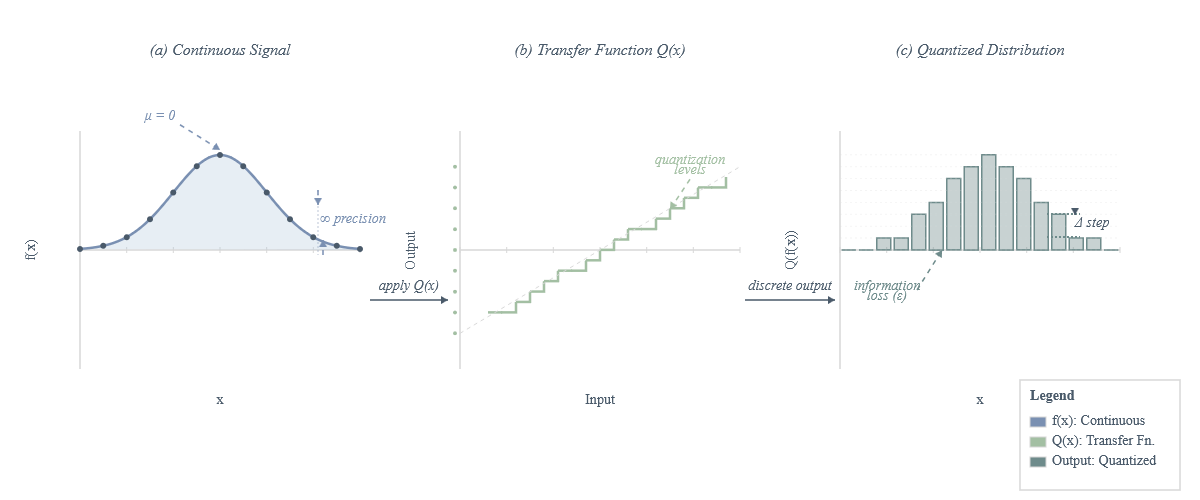
\includegraphics[scale=0.5]{quantization.png}%
  }
  \caption{Quantization of a normal distribution value $x$ into $n$ precision bits. The quantized value is computed as $Q(x) = \lfloor x \cdot 2^n \rfloor / 2^n$, and the quantization error $\varepsilon = |x - Q(x)|$}
  \label{fig:quantization_example}
\end{figure}

\subsection{Data Types used in Machine Learning}

\sunsubsection{Floating-Point Formats}

In the realm of deep learning training, the most prevalent floating-point formats are IEEE 754 Single Precision (FP32), Half Precision (FP16) \cite{micikevicius2017mixed}, and the Brain Floating Point (BFloat16 or BF16) \cite{kalamkar2019bfloat16}.

A floating-point number is structurally divided into bits allocated for the sign, the exponent, and the mantissa (significand). This structure allows for the representation of a vast range of values. Mathematically, a floating-point value $z$ is defined as:

\begin{equation}
  z = (-1)^s \times \left(1 + \frac{\hat{m}}{2^M}\right) \times 2^{\hat{e}-B}
  \label{eq:float}
\end{equation}

\noindent where $s$ represents the sign bit, $\hat{m}$ is the integer value of the mantissa comprising $M$ bits, $\hat{e}$ is the integer value of the exponent comprising $E$ bits, and $B$ is the exponent bias.

The trade-offs between these formats are visualized in Figure \ref{fig:dtypes} and summarized as follows:

\begin{itemize}
  \item \textbf{FP16:} By reducing the total bit count to 16, FP16 reduces memory bandwidth and storage requirements by $2\times$ compared to FP32. However, the reduced number of exponent bits shrinks the dynamic range, which can lead to numerical instability (e.g., underflow or overflow) during training.
  \item \textbf{BFloat16:} This format also provides a $2\times$ reduction in memory usage compared to FP32. Crucially, BFloat16 maintains the same number of exponent bits ($E=8$) as FP32, thereby preserving the full dynamic range of single-precision arithmetic \cite{kalamkar2019bfloat16}. This balance between the speed of half-precision and the range of single-precision makes BF16 a preferred standard for modern model training.
\end{itemize}

\begin{figure}[H]
  \centering
  \begin{tikzpicture}
    % Configuration
    \def\barheight{0.8}
    \def\totalwidth{12} % cm

    % FP32 Construction
    % 1 Sign, 8 Exp, 23 Mantissa = 32 total
    \node[anchor=west] at (0, 1.5) {\textbf{FP32} (32-bit)};

    % Sign
    \fill[signcol] (0,0) rectangle ++({1/32*\totalwidth}, \barheight);
    \node[white, font=\tiny] at ({0.5/32*\totalwidth}, \barheight/2) {S};

    % Exponent
    \fill[expcol] ({1/32*\totalwidth},0) rectangle ++({8/32*\totalwidth}, \barheight);
    \node[white, font=\tiny] at ({5/32*\totalwidth}, \barheight/2) {Exponent (8)};

    % Mantissa
    \fill[mantcol] ({9/32*\totalwidth},0) rectangle ++({23/32*\totalwidth}, \barheight);
    \node[white, font=\tiny] at ({20.5/32*\totalwidth}, \barheight/2) {Mantissa (23)};

    % Range vs Precision Arrow for FP32
    \draw[<->, gray] (0, -0.2) -- ({9/32*\totalwidth}, -0.2) node[midway, below, font=\tiny] {Range};
    \draw[<->, gray] ({9/32*\totalwidth}, -0.2) -- (\totalwidth, -0.2) node[midway, below, font=\tiny] {Precision};

    % BF16 Construction
    % 1 Sign, 8 Exp, 7 Mantissa = 16 total
    \begin{scope}[yshift=-2.5cm]
      \node[anchor=west] at (0, 1.5) {\textbf{BFloat16} (16-bit)};

      % Sign
      \fill[signcol] (0,0) rectangle ++({1/32*\totalwidth}, \barheight);
      \node[white, font=\tiny] at ({0.5/32*\totalwidth}, \barheight/2) {S};

      % Exponent (Same width as FP32)
      \fill[expcol] ({1/32*\totalwidth},0) rectangle ++({8/32*\totalwidth}, \barheight);
      \node[white, font=\tiny] at ({5/32*\totalwidth}, \barheight/2) {Exponent (8)};

      % Mantissa
      \fill[mantcol] ({9/32*\totalwidth},0) rectangle ++({7/32*\totalwidth}, \barheight);
      \node[white, font=\tiny] at ({12.5/32*\totalwidth}, \barheight/2) {Mant. (7)};

      % Empty space to show it is shorter
      \draw[dashed] ({16/32*\totalwidth},0) rectangle ++({16/32*\totalwidth}, \barheight);
      \node[gray, font=\tiny] at ({24/32*\totalwidth}, \barheight/2) {Saved Memory};
    \end{scope}

    % FP16 Construction
    % 1 Sign, 5 Exp, 10 Mantissa = 16 total
    \begin{scope}[yshift=-5cm]
      \node[anchor=west] at (0, 1.5) {\textbf{FP16} (16-bit)};

      % Sign
      \fill[signcol] (0,0) rectangle ++({1/32*\totalwidth}, \barheight);
      \node[white, font=\tiny] at ({0.5/32*\totalwidth}, \barheight/2) {S};

      % Exponent
      \fill[expcol] ({1/32*\totalwidth},0) rectangle ++({5/32*\totalwidth}, \barheight);
      \node[white, font=\tiny] at ({3.5/32*\totalwidth}, \barheight/2) {Exp (5)};

      % Mantissa
      \fill[mantcol] ({6/32*\totalwidth},0) rectangle ++({10/32*\totalwidth}, \barheight);
      \node[white, font=\tiny] at ({11/32*\totalwidth}, \barheight/2) {Mantissa (10)};

      % Empty space
      \draw[dashed] ({16/32*\totalwidth},0) rectangle ++({16/32*\totalwidth}, \barheight);
      \node[gray, font=\tiny] at ({24/32*\totalwidth}, \barheight/2) {Saved Memory};
    \end{scope}

  \end{tikzpicture}
  \caption{Visual comparison of bit allocation in FP32, BFloat16, and FP16 formats. Note that BFloat16 preserves the exponent width of FP32 to maintain dynamic range, while FP16 allocates more bits to the mantissa for precision at the cost of range.}
  \label{fig:dtypes}
\end{figure}

Once training concludes, models are often quantized by converting weights and activations from floating-point to integer representations, that is done to facilitate efficient deployment.

\subsubsection{Integer Formats}

Integer quantization is a critical technique for reducing model size and latency. The most widely adopted format is INT8 \cite{jacob2018quantization, dettmers2022gpt3int8}, followed by more aggressive compression formats like INT4 \cite{wu2023understanding}. Extreme quantization techniques can even reduce precision to binary formats \cite{hubara2016binarized}, yielding maximal reductions in memory footprint.

Integer formats utilize a simpler structural representation compared to floating-point numbers, enabling more efficient arithmetic logic units (ALUs). A quantized integer value is typically mapped to a real value using an affine transformation:

\begin{equation}
  z = s \times (\hat{z} - z_{zero})
  \label{eq:int}
\end{equation}

\noindent or, as often simplified in symmetric quantization schemes:

\begin{equation}
  z = s \times \hat{z} + b
\end{equation}

\noindent where $s$ is a strictly positive scale factor, $b$ is a bias term (related to the zero-point), and $\hat{z}$ represents the discrete integer value composed of $N$ bits (e.g., $N=8$ for INT8).

\begin{figure}[H]
  \centering
  \begin{tikzpicture}
    % Memory footprint comparison
    \begin{axis}[
        ybar,
        width=12cm,
        height=5cm,
        ylabel={Memory Footprint (Relative to FP32)},
        symbolic x coords={FP32, BF16, FP16, INT8, INT4, Binary},
        xtick=data,
        ymin=0, ymax=1.1,
        bar width=20pt,
        nodes near coords,
        nodes near coords align={vertical},
        title={Relative Memory Footprint by Data Type},
        legend pos=north east,
      ]
      \addplot[fill=signcol!70] coordinates {
        (FP32, 1.0)
        (BF16, 0.5)
        (FP16, 0.5)
        (INT8, 0.25)
        (INT4, 0.125)
        (Binary, 0.03125)
      };
    \end{axis}
  \end{tikzpicture}
  \caption{Relative memory footprint of different numerical formats normalized to FP32. Each reduction in bit-width yields proportional memory savings, with INT8 providing a 4× reduction and INT4 providing an 8× reduction compared to FP32.}
  \label{fig:memory_footprint}
\end{figure}

\subsection{Comparative Analysis}

Table \ref{tab:format_comparison} provides a comprehensive comparison of the key characteristics across different numerical formats used in machine learning.

\begin{table}[ht]
  \centering
  \caption{Comparison of Numerical Formats in Machine Learning}
  \label{tab:format_comparison}
  \begin{tabular}{@{}lcccccc@{}}
    \toprule
    \textbf{Format} & \textbf{Bits} & \textbf{Sign} & \textbf{Exp} & \textbf{Mant} & \textbf{Range} & \textbf{Primary Use} \\
    \midrule
    FP32   & 32 & 1 & 8  & 23 & $\pm$10$^{38}$ & Training (Legacy) \\
    BF16   & 16 & 1 & 8  & 7  & $\pm$10$^{38}$ & Training (Modern) \\
    FP16   & 16 & 1 & 5  & 10 & $\pm$10$^{5}$  & Training (Mixed) \\
    INT8   & 8  & - & -  & -  & [-128, 127]    & Inference \\
    INT4   & 4  & - & -  & -  & [-8, 7]        & Inference (Aggressive) \\
    Binary & 1  & - & -  & -  & \{-1, 1\}      & Extreme Compression \\
    \bottomrule
  \end{tabular}
\end{table}

\subsection{Hardware Considerations}

It is important to note that hardware support for these formats varies significantly across accelerator generations.
For instance, the NVIDIA V100 GPU based on the Volta architecture does not support native BFloat16 for its tensor cores, limiting mixed-precision options~\cite{datacrunch_v100_2025}.
In contrast, the NVIDIA H100 GPU (Hopper architecture) fully supports BFLOAT16 (and FP16, TF32, FP8, INT8) on its tensor cores, offering high throughput for modern AI workloads~\cite{nvidia_h100_specs_2025,nvidia_hopper_arch_in_depth_2022}.

Using a data format that the hardware does \emph{not} natively support typically forces software emulation (or fallback on “standard” CUDA cores), which can drastically degrade performance  negating the anticipated gains or even introducing computational bottlenecks~\cite{tensorrt_support_matrix_2025}.
Indeed, frameworks optimized for tensor-core use often disable certain precisions (e.g., BF16) on older GPUs.

Figure \ref{fig:hw_support} illustrates the evolution of data type support across different GPU architectures, highlighting the trend toward more diverse format support in recent generations.

\begin{figure}[ht]
  \centering
  \begin{tikzpicture}
    \begin{axis}[
        width=12cm,
        height=6cm,
        xlabel={GPU Architecture},
        ylabel={Supported Data Types},
        symbolic x coords={V100, A100, H100},
        xtick=data,
        ytick={0,1,2,3,4,5},
        yticklabels={0, FP32, +FP16, +TF32, +BF16, +INT8/4},
        grid=major,
        title={Hardware Data Type Support Evolution},
        legend pos=north west,
      ]

      % Cumulative support
      \addplot[ybar stacked, fill=signcol!70] coordinates {
        (V100, 1) (A100, 1) (H100, 1)
      };
      \addlegendentry{FP32}

      \addplot[ybar stacked, fill=mantcol!70] coordinates {
        (V100, 1) (A100, 1) (H100, 1)
      };
      \addlegendentry{FP16}

      \addplot[ybar stacked, fill=expcol!70] coordinates {
        (V100, 0) (A100, 1) (H100, 1)
      };
      \addlegendentry{TF32}

      \addplot[ybar stacked, fill=int8col!70] coordinates {
        (V100, 0) (A100, 1) (H100, 1)
      };
      \addlegendentry{BF16}

      \addplot[ybar stacked, fill=int4col!70] coordinates {
        (V100, 0) (A100, 1) (H100, 1)
      };
      \addlegendentry{INT8/4}

    \end{axis}
  \end{tikzpicture}
  \caption{Evolution of native hardware support for different data types across NVIDIA GPU architectures.}
  \label{fig:hw_support}
\end{figure}

\section{Fundamentals of Neural Network Pruning}

Neural network pruning is a model compression strategy aimed at reducing a network's complexity while preserving its performance. The term originates in horticulture, referring to the removal of excess growth of a plant or tree, and in computer science, it has long been associated with simplifying tree structures by removing redundant nodes and edges. This idea found early success in decision-tree learning, where pruning improves generalization by discarding superfluous branches~\cite{patil2010evaluation,aksoy2005rules3}. Because feed-forward neural networks can be represented as directed acyclic graphs, this intuition is directly transferable: unnecessary connections or entire units can be removed without altering the network's fundamental structure. In practice, pruning removes individual parameters or structured groups of parameters, thereby reducing the model's memory footprint and computational cost~\cite{cheng2025survey,nguyen2017nettrim}. While a fully trained, dense model may achieve peak training performance, pruning presents a trade-off: it can potentially boost generalization by removing redundant complexity, or, in the worst case, cause a noticeable drop in performance metrics such as accuracy or perplexity.

The primary objective of pruning is to introduce sparsity into the weight matrices $\mathbf{W}$ of a neural network. A matrix $\mathbf{W}$ is defined as $p$-sparse if a fraction $p$ of its elements are zero. The effectiveness of this sparsity is measured using multiple metrics beyond simple accuracy. These include the \textbf{Parameter Count ($P$)}, where $P = \sum_{i,j} \mathbb{I}[W_{i,j} \neq 0]$ directly correlates to memory footprint; \textbf{Floating Point Operations (FLOPs)}, quantified by the reduction ratio $R_{\text{FLOP}}$; \textbf{Inference Latency ($\mathcal{L}_{\text{inf}}$)}, measuring the actual time required for inference on target hardware; and \textbf{Perplexity (PPL)}, the standard language modeling metric defined as $\exp(\mathcal{L})$.

To frame this theoretically, let $f(\cdot;\Theta)$ be a neural network with parameters $\Theta$, and $L(\Theta) = \mathbb{E}_{(x,y)\sim p}[c(f(x;\Theta),y)]$ be the expected risk. Pruning aims to obtain a sparse parameter matrix $\Theta'$ that retains the predictive performance of the dense model. This is classically formulated as a constrained optimization problem:
\begin{equation}
\label{eq:pruning_constrained}
\min_{\Theta'} \;\widehat L(\Theta')
\qquad \text{s.t.}\qquad
\|\Theta'\|_{0} \le B,
\end{equation}
where the $\ell_0$ ``norm'' counts the nonzero entries and $B$ is a sparsity budget. This constraint is typically implemented via a binary mask $M \in \{0,1\}^{n\times m}$ such that $\Theta' = M \odot \Theta$, where $\odot$ denotes the Hadamard product. Consequently, pruning becomes the search for an optimal mask $M$.

However, pruning does not naturally correspond to a single objective; it requires balancing performance degradation against sparsity levels. Treating this as a multi-objective problem leads to the concept of \emph{Pareto optimality}. A candidate solution $\Theta'$ is Pareto optimal if no other valid solution improves sparsity without worsening loss, or improves loss without reducing sparsity. The set of all such solutions forms the \emph{Pareto front}, representing the optimal trade-off curve. To make this computationally tractable, the problem is often reduced via linear scalarization:
\begin{equation}
\label{eq:scalarization}
\min_{\Theta'}\;
\lambda_{\mathrm{perf}}
\big(\widehat L(\Theta') - \widehat L(\Theta)\big)
+
\lambda_{\mathrm{spar}}\|\Theta'\|_0,
\end{equation}
where varying the weights $\lambda_{\mathrm{perf}}$ and $\lambda_{\mathrm{spar}}$ allows one to trace different operating points along the Pareto frontier.

In implementation, pruning methods generally diverge into two main branches: \textbf{Unstructured} and \textbf{Structural} pruning~\cite{he2023structured,gale2019state}. Unstructured pruning involves removing individual weights $W_{i,j}$ (setting them to zero). While this approach can achieve substantially higher sparsity (often 95\%+), the resulting irregular data access patterns often prevent commodity hardware from capitalizing on the reduced FLOP count to achieve proportional speedups~\cite{frankle2018lottery,han2015deep}. Conversely, Structural pruning removes contiguous groups of parameters, such as entire neurons, filters, attention heads, or blocks~\cite{ma2023llmpruner,sun2023simple}. This regularity allows for efficient acceleration on standard GPUs or CPUs, leading to tangible improvements in inference latency, albeit typically at lower sparsity levels (40\%--70\%) compared to unstructured methods. Table~\ref{tab:pruning_comparison} summarizes these operational trade-offs.

\begin{table}[H]
\centering
\caption{Foundational Comparison of Pruning Granularity}
\label{tab:pruning_comparison}
\begin{tabular}{@{}p{2.2cm}p{2.5cm}p{2cm}p{2.5cm}p{2.5cm}@{}}
\toprule
\textbf{Pruning Type} & \textbf{Target Unit} & \textbf{Hardware Accel.} & \textbf{Sparsity Potential} & \textbf{Optimization Focus} \\ \midrule
Unstructured & Individual Weight $W_{i,j}$ & Low (Irregular) & High (95\%+) & Model Size, Memory \\
Structural (SRP) & Neuron, Head, Filter, Block & High (Regular) & Moderate (40\%-70\%) & Inference Speedup, FLOPs \\ \bottomrule
\end{tabular}
\end{table}

\begin{figure}[H]
    \centering
    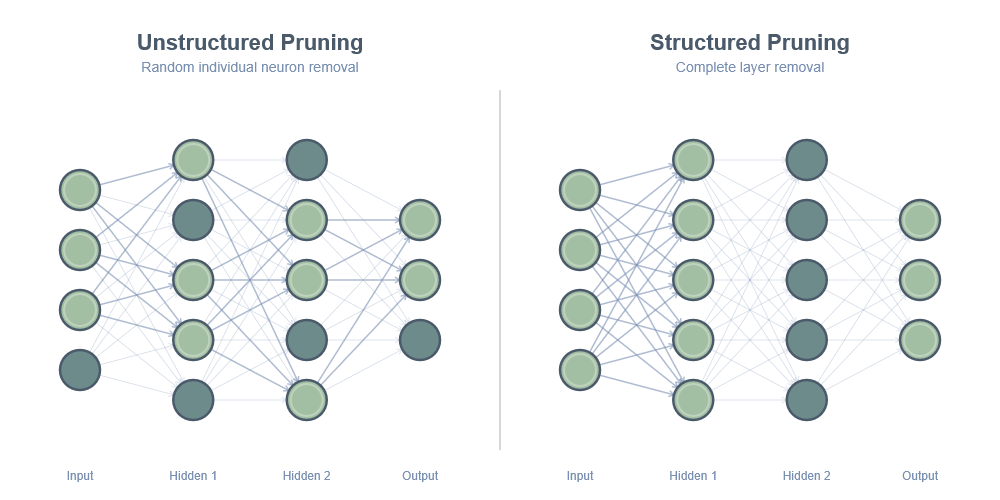
\includegraphics[scale=0.4]{canvas.png}
    \caption{The difference between unstructured pruning and structured pruning; the former removes individual neurons or weights, while the latter removes entire layers or structural blocks.}
    \label{fig:unstructured_vs_structured}
\end{figure}


\section{Low-Rank Factorization}

Low-rank factorization is a matrix decomposition technique that approximates high-dimensional matrices as products of lower-dimensional counterparts. The fundamental principle driving this approach is that deep neural network weights often exhibit significant redundancy and can be well-approximated by matrices of lower rank without a significant loss in representational capacity. This theoretical foundation was established by Li et al.~\cite{li2018measuring}, who demonstrated that the optimization landscape of deep networks is constrained to a low-dimensional manifold. In the context of large language models (LLMs), Aghajanyan et al.~\cite{aghajanyan2020intrinsic} further showed that this ``intrinsic dimensionality'' effectively predicts the success of fine-tuning regimes. When applied to architectures like the Transformer~\cite{vaswani2017attention}, low-rank factorization replaces a large weight matrix $W \in \mathbb{R}^{m \times n}$ with the product of smaller matrices $A \in \mathbb{R}^{m \times r}$ and $B \in \mathbb{R}^{r \times n}$, where $r \ll \min(m,n)$, such that:
\begin{equation}
  W \approx AB.
  \label{eq:lowrank_basic}
\end{equation}

The primary advantages of this decomposition are a reduced parameter count and a smaller memory footprint. While the original matrix requires $mn$ parameters, the factorized form requires only $r(m+n)$. As noted in the survey by Tay et al.~\cite{tay2020efficient}, this reduction is critical for deploying Transformers on memory-constrained devices, as reduced memory traffic alleviates bandwidth bottlenecks, a major performance limiter identified in works such as FlashAttention~\cite{dao2022flashattention}. The compression efficiency can be quantified by the ratio $\frac{mn}{r(m+n)}$. For instance, with dimensions $m = n = 4096$ and a rank $r = 64$, the compression ratio approaches $32\times$. However, the choice of rank $r$ introduces a fundamental trade-off between compression and model capacity. This balance is the central focus of parameter-efficient fine-tuning (PEFT) methods, most notably LoRA (Low-Rank Adaptation)~\cite{hu2021lora}, and has recently been extended to quantized models like QLoRA~\cite{dettmers2023qlora}, enabling the fine-tuning of massive parameter models on consumer hardware.

From a mathematical perspective, factorization is treated as an optimization problem minimizing the reconstruction error between the dense weight and its low-rank approximation. Formally, for a target rank $r$, we seek matrices $A$ and $B$ that minimize a distance metric, typically the Frobenius norm:
\begin{equation}
  \min_{A,B} \|W - AB\|_F^2.
  \label{eq:factorization_opt}
\end{equation}
While optimal factors correspond to the truncated Singular Value Decomposition (SVD), modern probabilistic algorithms allow for efficient computation even for massive matrices~\cite{halko2011finding}. In the specific context of Self-Attention, Wang et al.~\cite{wang2020linformer} proved in \textit{Linformer} that the attention matrix is inherently low-rank, justifying approximations that reduce complexity from $O(N^2)$ to $O(N)$. Similarly, Choromanski et al.~\cite{choromanski2020rethinking} utilized kernel-based approximations in the \textit{Performer} architecture. In modern fine-tuning scenarios, Hu et al.~\cite{hu2021lora} modified this formulation by freezing the pre-trained weights $W_0$ and learning a low-rank update $\Delta W = AB$, such that the forward pass becomes $h = W_0 x + ABx$. The success of these methods depends on rank selection; research by Ganesh et al.~\cite{ganesh2021compressing} suggests that different Transformer layers possess varying sensitivities to rank reduction, advocating for adaptive rather than uniform rank selection to minimize the normalized reconstruction error $\mathcal{E}(r) = \|W - \hat{W}_r\|_F / \|W\|_F$.

% Define colors for the TikZ figure if not already defined in preamble
\definecolor{mistyblue}{RGB}{173, 216, 230}
\definecolor{sagegreen}{RGB}{135, 175, 135}
\definecolor{dustyteal}{RGB}{95, 158, 160}
\definecolor{decompcol}{RGB}{25, 25, 112} % MidnightBlue
\definecolor{lowrankcol}{RGB}{47, 79, 79} % DarkSlateGray

\begin{figure}[h!]
  \centering
  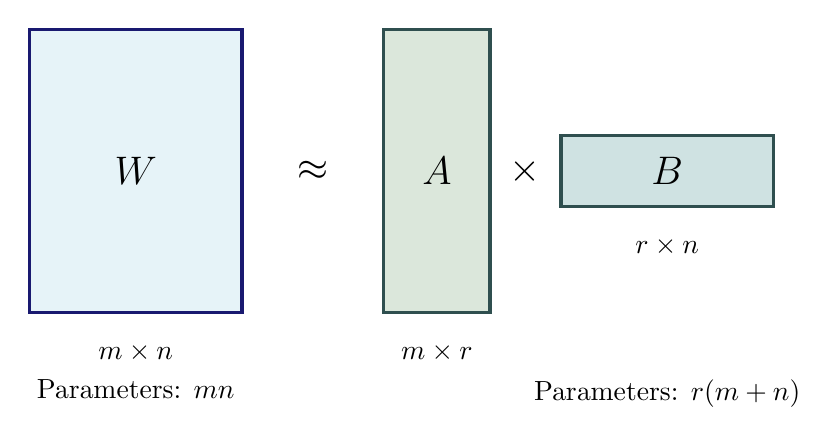
\begin{tikzpicture}[scale=0.9]
    % Original matrix
    \draw[fill=mistyblue!30, draw=decompcol, very thick] (0,0) rectangle (3,4);
    \node at (1.5,2) {\Large $W$};
    \node[below] at (1.5,-0.3) {$m \times n$};
    \node[below] at (1.5,-0.8) {Parameters: $mn$};

    % Approximately equal
    \node at (4,2) {\Large $\approx$};

    % First factor
    \draw[fill=sagegreen!30, draw=lowrankcol, very thick] (5,0) rectangle (6.5,4);
    \node at (5.75,2) {\Large $A$};
    \node[below] at (5.75,-0.3) {$m \times r$};

    % Multiplication
    \node at (7,2) {\Large $\times$};

    % Second factor
    \draw[fill=dustyteal!30, draw=lowrankcol, very thick] (7.5,1.5) rectangle (10.5,2.5);
    \node at (9,2) {\Large $B$};
    \node[below] at (9,1.2) {$r \times n$};

    % Annotation
    \node[below] at (9,-0.8) {Parameters: $r(m+n)$};
  \end{tikzpicture}
  \caption{Low-rank factorization approximates a weight matrix $W$ as a product of two smaller matrices $A$ and $B$. This structure is utilized in ALBERT \cite{lan2019albert} and LoRA \cite{hu2021lora}.}
  \label{fig:lowrank_concept}
\end{figure}






